\documentclass[11pt]{article}
\usepackage[T1]{fontenc}
\usepackage[margin=1in]{geometry}
\usepackage{amsmath}
\usepackage{tikz}
\usetikzlibrary{arrows.meta, shapes.geometric, positioning, calc, fit, backgrounds, decorations.pathmorphing}

\title{South Campus Sensor Network: Gateway Placement Study}
\author{Facilities Engineering, Network Planning Group}
\date{October 2026}

\begin{document}
\maketitle

\section{Introduction}
This note documents the proposed placement of wireless gateways for the
south campus environmental sensor network. Each building in the pilot
area carries a pair of field probes---one temperature probe and one
humidity probe---that report over a low-power radio link to a
building-level gateway. The gateways forward readings over the wired
backbone to a central collector, which archives them for the building
management system.

The pilot covers twelve buildings, but the topology repeats: every
building instantiates the same four-node pattern shown in
Figure~\ref{fig:topology}. The only per-building parameters are the
radio distances, which range from 8 to 40 metres, and the reporting
interval, which is five minutes for temperature and fifteen minutes
for humidity.

\section{Network Layout}
Figure~\ref{fig:topology} shows the reference pattern. The two field
probes sit at the top; the wavy edges denote the wireless hop to the
gateway, drawn here with a snake decoration to distinguish it from the
wired links. The gateway aggregates both streams and forwards them to
the collector over Ethernet. The dashed outline groups the field
cluster, while the shaded backdrop marks the equipment that lives in
the building wiring closet.

\begin{figure}[htbp]
\centering
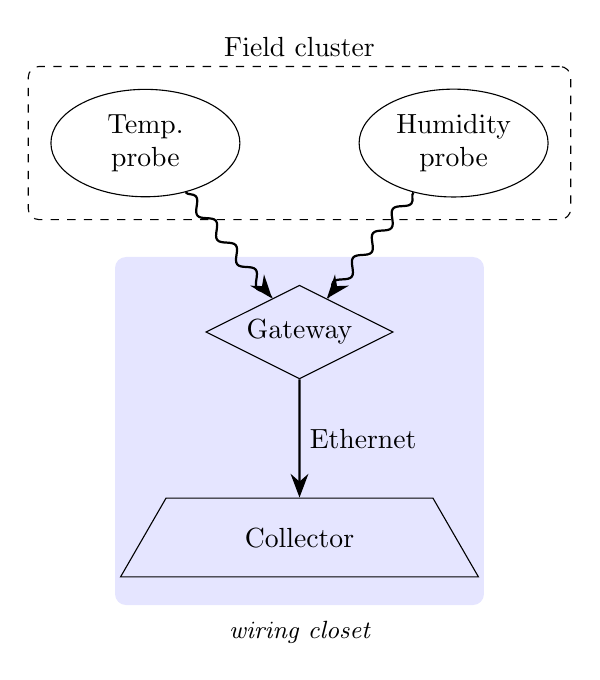
\begin{tikzpicture}[
  node distance=1.5cm,
  sensor/.style={draw, ellipse, minimum width=2.4cm, minimum height=1cm, align=center},
  gateway/.style={draw, diamond, aspect=2, align=center, inner sep=2pt},
  server/.style={draw, trapezium, minimum width=2.8cm, minimum height=1cm, align=center},
  wire/.style={-{Stealth[length=3mm]}, thick},
  radio/.style={-{Stealth[length=3mm]}, thick, decorate, decoration={snake, amplitude=0.7mm, segment length=4mm}},
]
\node[sensor] (temp) {Temp.\\probe};
\node[sensor, right=of temp] (hum) {Humidity\\probe};
\node[gateway] (gw) at ($(temp)!0.5!(hum) + (0,-2.4)$) {Gateway};
\node[server, below=of gw] (srv) {Collector};
\draw[radio] (temp) -- (gw);
\draw[radio] (hum) -- (gw);
\draw[wire] (gw) -- node[right] {Ethernet} (srv);
\node[draw, dashed, rounded corners, fit=(temp) (hum), inner sep=8pt,
  label={above:Field cluster}] (field) {};
\begin{scope}[on background layer]
  \node[fill=blue!10, rounded corners, fit=(gw) (srv), inner sep=10pt] (closet) {};
\end{scope}
\node[below=2pt of closet, font=\small\itshape] {wiring closet};
\end{tikzpicture}
\caption{Reference four-node topology, repeated in every pilot building.}
\label{fig:topology}
\end{figure}

The midpoint construction in the diagram is deliberate: the gateway is
centred horizontally between its two probes, so the radio diagram stays
symmetric whatever the probe spacing. Distances were surveyed in
September; the longest wireless hop is 38 metres through two interior
walls, which bench tests show still leaves 12~dB of link margin.

\section{Findings}
The study recommends one gateway per building, mounted in the wiring
closet beside the collector uplink. The measured packet delivery rate
over two weeks was 99.7~\%, with all losses confined to a single
gateway whose antenna was later found misaligned. Re-aiming the
antenna cleared the errors, and no losses have been observed since.

Total hardware cost for the pilot is twelve gateways plus the
collector VM, well inside the project budget. The next step is to
extend the same pattern to the north campus residences, where the
longer inter-building distances may require an additional relay hop;
that extension will be the subject of a follow-up note.
\end{document}
